\chapter{Wykorzystane oprogramowanie}
\section{Eclipse}

\section{ANTLR}
ANTLR (ang. \emph{ANother Tool for Language Recognition}) jest generatorem
analizatorów leksykalnych i składniowych \cite{antlr}.

Narzędzie przetwarza opisy gramatyk języków formalnych w postaci 
zbliżonej do notacji
 Backusa-Naura. Na podstawie specyfikacji generowany jest kod analizatora.
Językami programowania wspieranymi przez ANTLR są między innymi C, C\#, Java
i Python.

Istotną zaletą oprogramowania jest jego prostota użycia. Wygenerowany kod 
jest czytelny i łatwo można go dołączyć do własnej aplikacji. Postać plików
wejściowych jest podobna dla wszystkich rodzajów analizatorów. Dodatkowo
istnieją narzędzia wspierające projektowanie i implementację gramatyk
formalnych z wykorzystaniem ANTLR. Należy do nich ANTLRWorks, będące
zintegrowanym środowiskiem programistycznym. Zawiera ono edytor strukturalny,
zintegrowany program do usuwania błędów i moduł do wizualizacji struktur 
danych powstających podczas translacji.

ANTLR został opublikowany wraz z kodem źródłowym na licencji BSD. Projekt jest
aktywnie rozwijany. Wiele programów zawiera analizatory wygenerowane za pomocą
ANTLR. Należą do nich Hibernate, Jython i Netbeans.

\subsection{Przetwarzanie języków formalnych}
Języki formalne, w tym języki programowania, są opisane zbiorem zasad określającym
ich składnię i semantykę. Analiza języka formalnego polega na sprawdzeniu zgodności
danych wejściowych ze specyfikacją języka oraz na wyodrębnieniu części składniowych.
Ponadto podczas analizy mogą zostać wykonane operacje działające na danych zgodnie
z ich znaczeniem określonym przez reguły semantyczne \cite{compilers}.

Wyodrębnia się trzy fazy analizy:
\begin{enumerate}
\item \emph{Analizę leksykalną}.
\item \emph{Analizę składniową}.
\item \emph{Analizę semantyczną}.
\end{enumerate}

\begin{figure}[h]
  \centering
    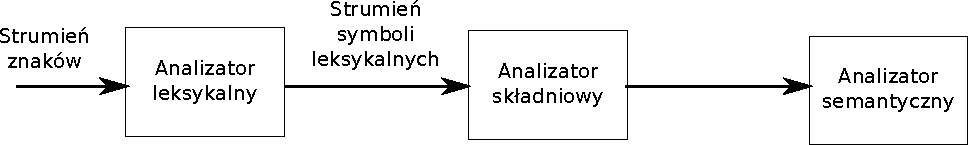
\includegraphics[width=\textwidth]{img/antlr_phases.pdf}
    \caption{Fazy analizy języka formalnego}
    \label{antlr_phases}
\end{figure}

Zależności pomiędzy fazami przedstawia rysunek \ref{antlr_phases}. 

Podczas analizy leksykalnej dane wejściowe są traktowane jako strumień znaków, który
jest odczytywany od strony prawej do lewej. Znaki są grupowane w \emph{symbole leksykalne}, czyli
ciągi posiadające określone znaczenie. Analiza składniowa ma na celu zgrupowanie 
symboli leksykalnych w hierarchiczne struktury,
mające pewne znaczenie. Analiza semantyczna przetwarza dane zgodnie z ich znaczeniem
opisanym przez reguły semantyczne. W tej fazie zbierane są informacje zawarte w danych.

Reguły języka mogą być opisane językiem naturalnym lub w sposób sformalizowany.
Jednym z formalizmów, odzwierciedlającym hierarchiczną strukturę konstrukcji językowych,
jest \emph{gramatyka bezkontekstowa}. Składa się ona z czterech elementów:

%Pytanie nieuniknięto powtórzenia skłów w definicji
\begin{itemize}
\item Zbioru symboli leksykalnych zwanych \emph{symbolami terminalnymi} lub \emph{terminalami}.
\item Zbioru symboli \emph{nieterminalnych}.
\item Zbioru \emph{produkcji}. Każda produkcja składa się z symbolu nieterminalnego,
  zwanego lewą stroną produkcji, strzałki i ciągu symboli zwanego prawą stroną produkcji.
\item Wyznaczonego \emph{symbolu startowego}.
\end{itemize}

Mówi się, że gramatyka wyprowadza ciąg symboli leksykalnych, jeżeli wychodząc 
od symbolu startowego i zamieniając symbole nieterminalne na ciągi znajdujące 
się po prawych stronach produkcju, można otrzymać dany ciąg. Sposób, w jaki
można wyprowadzić dany napis obrazuje \emph{drzewo wyprowadzania}. W korzeniu drzewa wyprowadzania
znajduje się symbol startowy. Dzieci wierzchołka reprezentującego symbol nieterminalny
zawierają symbole z prawej strony produkcji użytej do jego zastąpienia.

\paragraph{Przykład 4.1}
Rozpatrzmy przykład konstrukcji języka PDDL reprezentującej listę wymagań domeny lub problemu.
Składa się ona z otoczonych nawiasami okrągłymi symbolu \texttt{:requirements} oraz
ciągu symboli oznaczających nazwy wymagań. Symbolami terminalnymi są 
\textbf{(}, \textbf{)}, słowo kluczowe \textbf{:requirements} i 
\textbf{requirementName} reprezentujący nazwę wymagania. Poniższa gramatyka opisuje
składnię takiego wyrażenia:

\begin{itemize}
\item requirementsList $\rightarrow$ \textbf{(} \textbf{:requirements} R
\item R $\rightarrow$ \textbf{requirementName} \textbf{)}
\item R $\rightarrow$ \textbf{requirementName} \textbf{R}
\end{itemize}

Dla napisu postaci \texttt{(:requirements :strips)} zostanie
wygenerowany strumień symboli leksykalnych \textbf{( :requirements requirementName )}.
Drzewo wyprowadzania tworzone podczas analizy składniowej jest przedstawione 
na rysunku \ref{antlr_example}

\begin{figure}[h!]
  \centering
    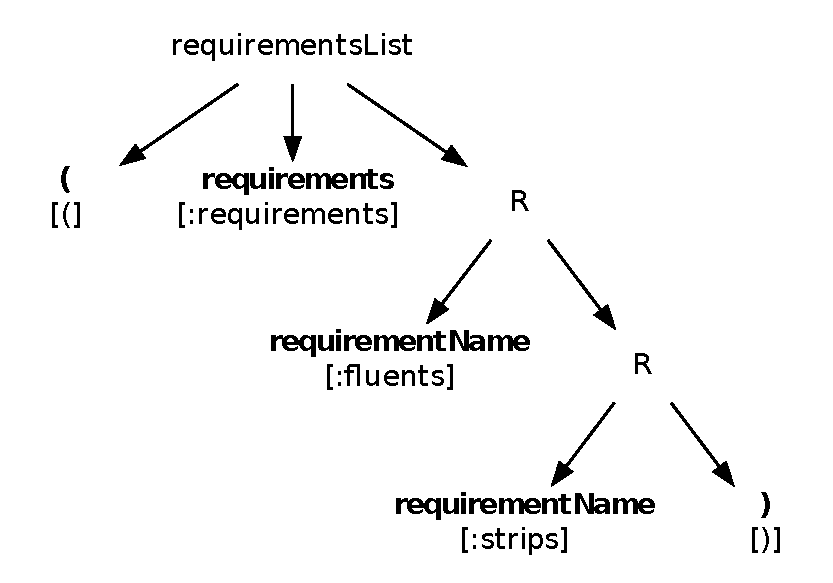
\includegraphics[width=0.7\textwidth]{img/antlr_example.pdf}
    \caption{Drzewo wyprowadzania dla przykładu 12}
    \label{antlr_example}
\end{figure}

\subsection{Metoda LL(*)}
Główną zaletą gramatyk bezkontekstowych jest możliwość automatycznego generowania programów
wykonujących analizę leksykalną i składniową na podstawie gramatyki.

Narzędzie ANTLR generuje analizatory leksykalne i składniowe dla pewnego podzbioru
gramatyk formalnych. Elementy tego podzbioru nazwane są gramatykami LL(*). Metoda 
analizy stosowana w generowanych analizatorach nazwana jest analizą LL(*). 

Analizatory LL(*) należą do klasy analizatorów LL. Wykorzystują one
analizę zstępującą i metodę zejść 
rekurencyjnych. Każdemu nieterminalowi zdefiniowanemu w specyfikacji gramatyki
odpowiada procedura lub metoda. 

Analiza, polegająca na konstrukcji drzewa
wyprowadzenia, rozpoczyna się od korzenia. Związany z nim jest symbol 
startowy gramatyki. W każdym kroku analizy wykonywane są następujące czynności:
\begin{enumerate}
\item wybierany jest pierwszy w porządku zdefiniowanym przez
  przeszukiwanie wgłąb węzeł V zawierający symbol nieterminalny A.
\item wybierana jest produkcja mająca po lewej stronie symbol A.
\item dodawane są węzły związane z symbolami znajdującymi się po prawej
  stronie produkcji z punktu 2. Stają się one dziećmi węzła V.
\end{enumerate}

Typy analizatorów należących do klasy LL różnią się sposobem wyboru produkcji w punkcie 2. 
Analizatory LL(*) są analizatorami przewidującymi. Podejmują one decyzję na
podstawie nieprzetworzonych symboli leksykalnych w strumieniu wejściowym. Liczba
tych symboli nie jest ograniczona. W celu przeglądania strumienia wejściowego 
,,w przód'' tworzone są automaty skończone mogące zawierać cykle.

W odróżnieniu od tradycyjnych gramatyk LL, W gramatykach LL(*) prawe strony
produkcji dla jednego nieterminala mogą mieć ten sam prefiks. Nie ma więc 
konieczności lewostronnej faktoryzacji, co znacznie ułatwia tworzenie
gramatyk.

\subsection{Abstrakcyjne drzewa składniowe}
% Analizę semantyczną języka opisanego gramatyką bezkontekstową można 
% sprowadzić do obliczania wartości atrybutów przyporządkowanych symbolom
% znajdującym się w drzewie wyprowadzanie. Produkcjom przypisywane są 
% wówczas reguły określające wartości atybutów. Takie podejście 

Formą pośrednia przekazywaną pomiędzy analizatorem składniowym a semantycznym
może być \emph{abstrakcyjne drzewo składniowe}. Jest to skondensowana postać drzewa
wyprowadzania, skłądająca się
wyłącznie z węzłów reprezentujących symbole wejściowe. Węzły
wewnętrzne reprezentują słowa kluczowe i operatory, liście -- argumenty.
Abstrakcyjne drzewo składniowe dla przykładu 1 jest przedstawione na rysunku 
\ref{antlr_ast}.

\begin{figure}[h!]
  \centering
    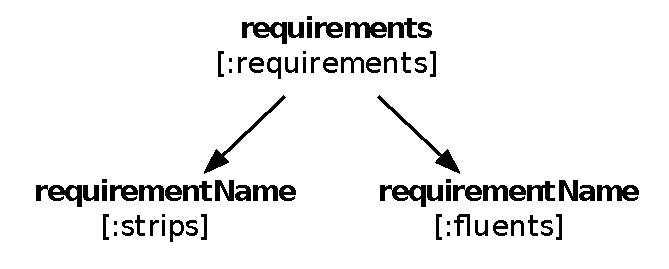
\includegraphics[scale=0.8]{img/antlr_ast.pdf}
    \caption{Abstrakcyjne drzewo składniowe dla przykładu 1}
    \label{antlr_ast}
\end{figure}

%Przykład drzewa

Możliwe jest ręczne tworzenie drzewa składniowego za pomocą odpowiednich
reguł semantycznych. Takie podejście proceduralne jest opisane w \cite{compilers}.

Narzędzie ANTLR wspiera tworzenie drzew składniowych. Dodanie
odpowiedniej opcji w specyfikacji analizatora składniowego powoduje automatyczne
wygenerowanie struktury. Poza tym, specyfikacja analizatora składniowego
 może zawierać elementy deklaratywne wpływające na kształt drzewa.


Przetwarzanie abstrakcyjnego drzewa składniowego podczas analizy semantycznej
sprowadza się do jego przechodzenia. Można do tego wykorzystać analizator drzewowy. 
Jest to podprogram generowany przez
ANTLR na podstawie specyfikacji, tak jak analizator składniowy lub leksykalny.
Wprowadzenie analizatorów drzewowych wyróżnia ANTLR na tle innych generatorów
 parserów. 

\subsection{Pliki wejściowe}

Pliki wejściowe ANTLR posiadają rozszerzenie .g. Zawierają one specyfikację
analizatora leksykalnego, składniowego, drzewowego lub połączoną specyfikację
analizatorów leksykalnego i składniowego. 

Specyfikacja analizatorów składa się z listy produkcji, definiujących symbole,
 sekcji opcji konfiguracyjnych oraz kodu dodawanego do generowanego
pliku źródłowego.

W przypadku plików zawierających połączoną specyfikację analizatorów, występuje
podział symboli ze względu na pierwszą literę ich nazwy.
 Symbole, których nazwa rozpoczyna się wielką literą uznawane są
za symbole terminalne. W ich definicjach mogą występować literały i inne
symbole terminalne. Na podstawie reguł definiujących symbole terminalne
tworzony jest analizator leksykalny. Pozostałe reguły tworzą analizator
składniowy.

